\section{Overcomplete Dictionaries}
\subsection{Introduction}
\emph{Overcompleteness} $(L>D)$: More atoms (dictionary elements) than dimensions.

\subsection{Morphology of Signals}
Different dictionaries are appropriate for different kinds of signals.

\paragraph{Dictionary selection Strategy} Either choose the appropriate dictionary manually or try several and choose the one which affords sparsest coding.

\subsubsection{Unions of Bases} 
\emph{Union of orthonormal bases} $[U_1\ldots U_B] \in \R^{D\times (B\cdot D)}$
\begin{figure}[H]
    \centering
    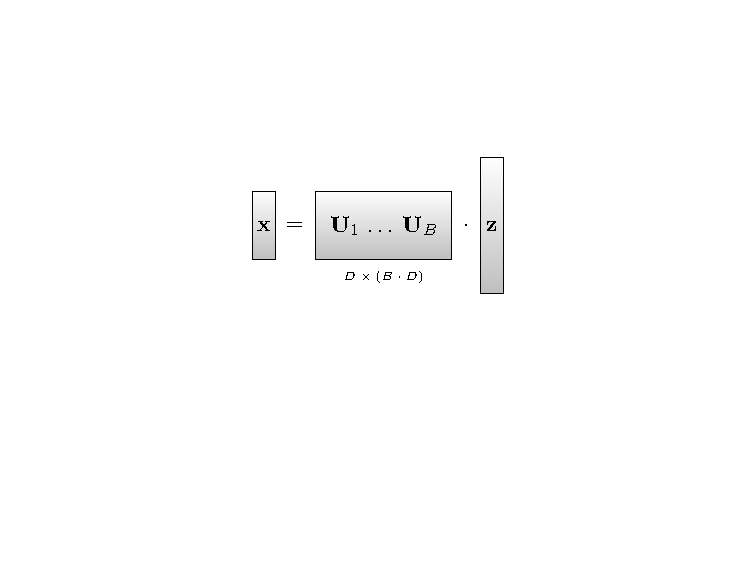
\includegraphics[width=0.6\textwidth]{img/09_union_of_bases}
\end{figure}
Each basis $U_b$ is responsible for one characteristic of the signal, and the total number of atoms is $K=B\cdot D$.

\subsection{General Overcomplete Dictionaries}
Consider the data set $\{x_1,\ldots, x_{10000}\}\in \R^3$:
\begin{figure}[H]
    \centering
    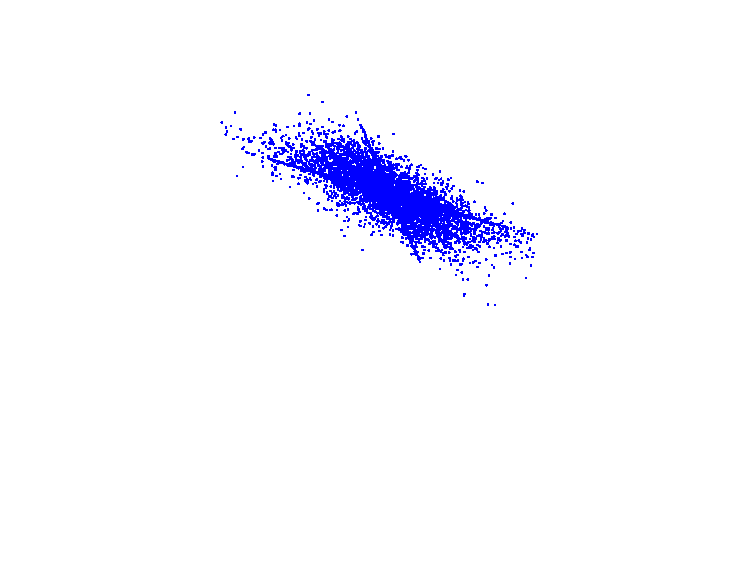
\includegraphics[width=0.6\textwidth]{img/09_overcomplete}
\end{figure}
\begin{itemize}
\item Full coding $(K=3)$ in spanning basis $U\in \R^{3\times 3}$.
\item $K=2$ coding possible using a four atom dictionary:
    \begin{align*}
         \tilde U = [u_1 u_2 u_3 u_4]\in \R^{3\times 4}
    \end{align*}
    aligned with densely populated subspaces.
\item $L>D$ atoms are no longer linearly dependent.
\end{itemize}

\paragraph{Example: Directional Gabor Wavelets} Directional oscillation, amplitude modulated by Gaussian window:
\begin{align*}
    g(n_1, n_2; \mu_1, \mu_2,f\theta) \propto 
        \exp\left[ 
             -(n_1-\mu_1)^2
            \right]
        \exp\left[
                -(n_2-\mu_2)^2
            \right]
        \times \Re \left\{
                        \exp \left[
                                i\cdot f\cdot (n_1\cos\theta+n_2\sin\theta)
                            \right]
                    \right\}
\end{align*}
\begin{figure}[H]
    \centering
    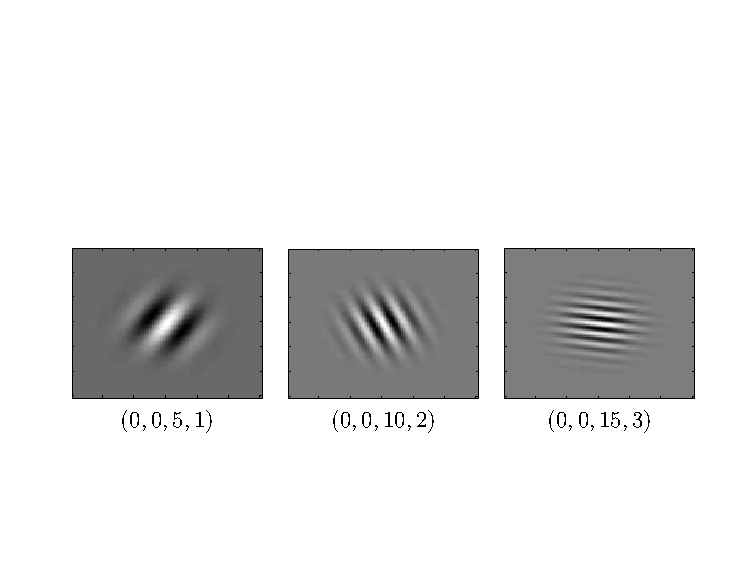
\includegraphics[width=0.8\textwidth]{img/09_gabor}
\end{figure}

\subsection{Coherence}
Increasing the \emph{over-completeness factor} ${L\over D}$:
\begin{itemize}
    \item Potentially increases the sparsity of the coding
    \item Increases the linear dependency betwee atoms.
\end{itemize}

Linear dependency measure for dictionaries: \emph{coherence}
\begin{align*}
    m(U) = \max_{i,j:\ i\neq j} \left| u_i^T u_j \right|
\end{align*}
\begin{description}
    \item $m(B)=0$ for an orthogonal basis $B$.
    \item $m([Bu]) \geq {1\over \sqrt{D}} $ if atom $u$ is added to $B$.
\end{description}

\subsection{Signal Coding}
\begin{description}
\item $U$ is \emph{orthonormal}:

    Matrix multiplication $z=U^T x$
\item $U$ is a \emph{spanning basis} ($D$ linearly dependent atoms):

    \begin{itemize}
        \item $z = U^{-1}$
        \item inverting $U$ can be ill-conditioned.
    \end{itemize}
\item $U \in \R^{D\times L}$ is \emph{overcomplete}:
    \begin{itemize}
        \item \emph{Ill-posed} problem: more unknowns than equations
        \item Have to add constraint: Find sparsest $z$ such that the equation holds:
            \begin{align*}
                 &z^* = \argmin_{z} \norm{z}_0\\
                 \text{s.t.}& x= Uz,
            \end{align*}
            where $\norm{z}_0$ counts the number of non-zero elements in $z$.
            
            \subitem $\norm{\cdot}_0$ is piece-wise constant.
            \subitem Finding the sparsest solution $z^*$ is NP hard (combinatorial problem).
            \subitem Brute-force approach: Try all possible atom subsets with $|\Delta| \leq D$.
            \subitem Needs an approximation scheme for realistic problem instances.
    \end{itemize}
\end{description}

\subsection{Noise Observations}
\subsubsection{Additive Noise}
\begin{align*}
     x = Uz + n
\end{align*}
Assumes each dimension is independently corrupted by zero-mean Gaussian nois:
    \begin{align*}
        n_d  \sim \mathcal N(0,\sigma^2)
    \end{align*}
    with variance $\sigma^2$.
    
\paragraph{Solve} by maximising the sparsity of $z$, while the \emph{residual} (approximation error) remains below $\sigma$:
\begin{align*}
     &z^*  = \argmin_{z} \norm{z}_0\\
     \text{s.t.}&\qquad \norm{x-Uz}_2 < \sigma
\end{align*}
or alternatively:

Minimise the residual while selecting less than $K$ atoms from the dictionary:
\begin{align*}
    &z^* = \argmin_z \norm{x-Uz}_2\\
    \text{s.t.}&\norm{z}_0 \leq K
\end{align*}

\subsubsection{Approximate Sparse Coding}
Explain the signal accurately with few atoms:
\begin{align*}
    x =Uz + n = Uz+Uy = U(z+y),    
\end{align*}
where $y$ is the coding of $n$ in $U$:
\begin{figure}[H]
    \centering
    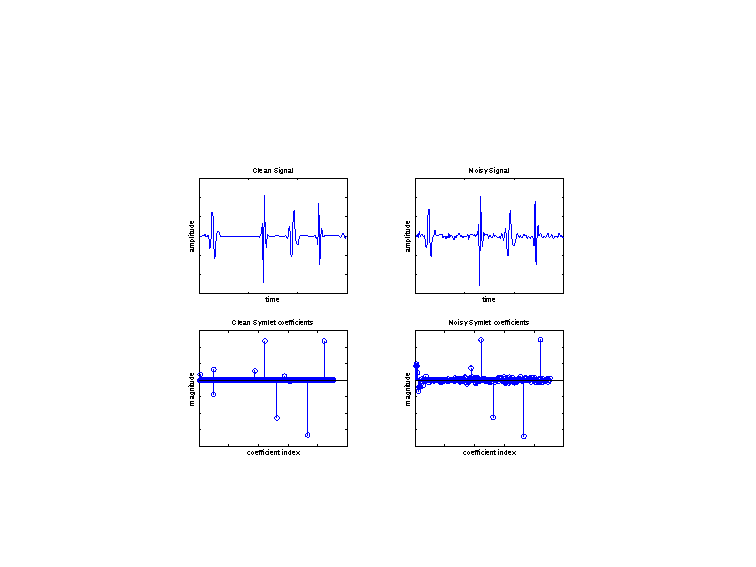
\includegraphics[width=0.7\textwidth]{img/09_noise_vs_signal}
\end{figure}
We observe that \emph{noise cannot be sparsely coded} in any dictionary, therefore $y$ has many small coefficients. Large coefficients are still due to $z$.

\paragraph{Geometry} of the sparse coding solution $z^*$:
\begin{figure}[H]
\centering
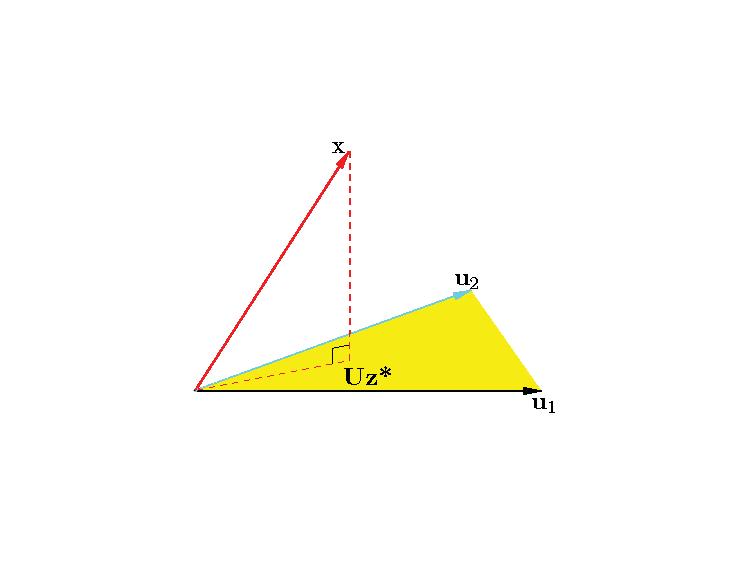
\includegraphics[width=0.5\textwidth]{img/09_geometry}
\end{figure}

The orthogonal projection of $x$ onto the subspace spanned by the selected atoms $\{u_d| z_d^* \neq 0\}$ minimises $\norm{x-Uz}_2$.

\section{Matching Pursuit}
Matching pursuit is a \emph{Greedy} algorithm: Thus approximates a NP hard problem iteratively each time taking the action which is short-term optimal.

\paragraph{Application to sparse coding:}$\ $
\begin{enumerate}
    \item Start with the zero vector $z=0$ and residual $r^0 = x$.
    \item At each iteration $t$, take a step in the direction of the atom $u_{d^*(t)}$ that maximally reduces the residual $\norm{x-Uz}_2$.
\end{enumerate}

\subsection{Minimising the Residual}
Atom selection at iteration $t$:
\begin{align*}
    d^{*} (t) = \argmax_d |\langle r^t, u_d\rangle|
\end{align*}

\paragraph{Proof} for the first iteration:
\begin{enumerate}
    \item Project $r^0 - x$ on atom $u_d$, to get
        \begin{align*}
            x = \langle x,u_d\rangle u_d + r^1
        \end{align*}
    \item Since $r^1$ is orthogonal to $u_d$, and $u_d^T u_d = 1$,
        \begin{align*}
            \norm{x}_2^2 = |\langle x,u_d\rangle|^2 + \norm{r^1}_2^2.
        \end{align*}
    \item Therefore, $\norm{r^1}_2^2$ is minimised by maximising $|\langle r^0, u_d\rangle|^2$.
\end{enumerate}



\subsection{Matching Pursuit Algorithm}
\begin{description}
\item[Objective] $\ $
    \begin{align*}
        z^* &= \argmin_z \norm{x-Uz}_2,\\
        \text{s.t }\ \norm{z}_0 &\leq K.
    \end{align*}

\item[Algorithm] $\ $
    \begin{algorithmic}
        \STATE $z\gets 0$
        \STATE $r\gets x$
        \WHILE{$\norm{z}_0 < K$}
            \STATE Select atom with maximum absolute correlation to residual:
                \begin{align*}
                 d^* \gets \argmax_d \left|  u_d^T r \right|
                \end{align*}
            \STATE Update coefficient vector and residual:
                \begin{align*}
                     z_{d^*} &\gets z_{d^*} + u_{d^*}^Tr\\
                     r &\gets r-\left( u_{d^*}^R r\right) u_{d^*}.
                \end{align*}
        \ENDWHILE
    \end{algorithmic}
\end{description}


\subsection{Discussion}
Assume $x=Uz$ has a $K$ sparse coding
\begin{align*}
 x=\sum_{d\in \Delta} z_d u_d.
\end{align*}

Under which condition is MP successful in recovering the true \emph{support}
\begin{align*}
    \Delta_{MP} = \Delta,
\end{align*}
where $\Delta_{MP} = \{d|z_{d^*} \neq 0\}$ is the set of coding atoms for the MP solution $z^*$?
Ie. when is the greedy approximation exact?

\begin{enumerate}
    \item Generate dictionary with atoms uniformly sampled on hypersphere.
    \item Generate observations with $K$ sparse coding.
\end{enumerate}
Compare $\Delta_{MO}$ with $\Delta$:

\begin{figure}[H]
    \centering
    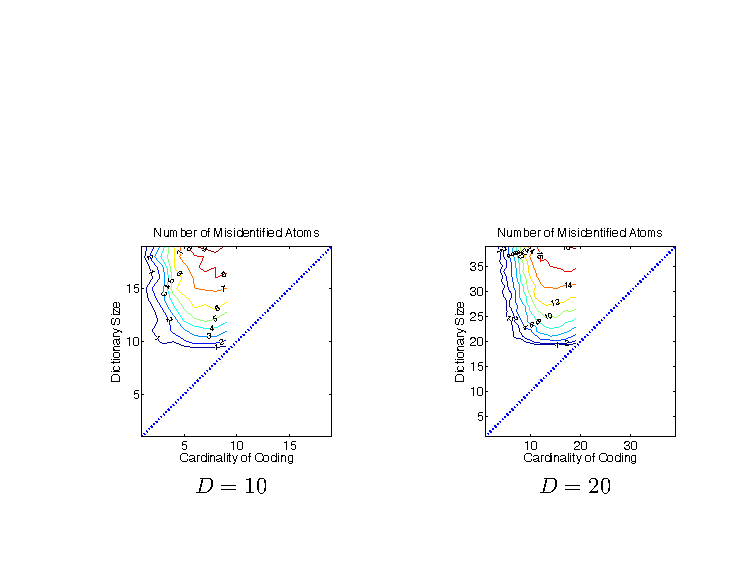
\includegraphics[width=0.7\textwidth]{img/09_mp_recovery}
\end{figure}
We observe that the recovery is possible even for $L>D$ if the true coding is \emph{sparse enough}.

\paragraph{Exact recovery condition}
    \begin{align*}
     K < {1\over 2} \left( 1+{1\over m(U)}\right)
    \end{align*}
guarantees support recovery by matching pursuit.


\begin{description}
\item Intuition: If the coherence is small, explaining a generating atom with other atoms is not sparse. Therefore sparse coding recovers support.
\item Trade-Off: Increasing L
    \begin{itemize}
        \item Leads to sparser coding (smaller possible $K$),
        \item But it increases coherence $m(U)$.
    \end{itemize}
\end{description}

\subsection{Inpainting}
\paragraph{Idea} $\ $
\begin{enumerate}
\item Sparse coding of known parts of the image,
\item Predicting missing parts by reconstruction from sparse code.
\end{enumerate}
\paragraph{Algorithm} $\ $
\begin{enumerate}
    \item Define a diagonal masking matrix $M$, $m_{d,d} = 1$ if pixel $d$ is known, $m_{d,d} = $ if pixel $d$ is missing.
    \item Sparse coding of known parts in over-complete dictionary $U$:
    \begin{align*}
        z^* &= \min_z \norm{z}_0\\
        \text{s.t. }\ &\norm{M(x-Uz)}_2 < \sigma.
    \end{align*}
    \item Image reconstruction using mask:
    \begin{align*}
        \hat x = Mx + (I-M)Uz^*.
    \end{align*}
\end{enumerate}
\paragraph{Iterative EM Algorithm} $\ $
\begin{enumerate}
\item Assume initial sparse coding $z^0$ of image.
\item Reconstruct image using mask
\begin{align*}
    x^1 = Mx + (I-M)Uz^0.
\end{align*}
\item Sparse coding of reconstructed image $x^1$:
    \begin{align*}
        z^1 &= \min_z \norm{z}_0\\
        \text{s.t. }\ &\norm{x^1-Uz}_2 <\sigma.
    \end{align*}
\item Iterate steps (2.) and (3.) $t$ times until convergence.
\item Image reconstruction using mask:
    \begin{align*}
        \hat x = Mx + (I-M)x^t.
    \end{align*}
\end{enumerate}








































